\section{5.3 Applications: Order-finding and Factoring}

The phase estimation procedure can be used to solve a variety of interesting problems. We now describe two of the most interesting of these problems: the order-finding problem, and the factoring problem. These two problems are, in fact, equivalent to one another, so in Section 5.3.1 we explain a quantum algorithm for solving the order-finding problem, and in Section 5.3.2 we explain how the order-finding problem implies the ability to factor as well.

To understand the quantum algorithms for factoring and order-finding requires a little background in number theory. All the required materials are collected together in Appendix 4. The description we give over the next two sections focuses on the quantum aspects of the problem, and requires only a little familiarity with modular arithmetic to be readable. Detailed proofs of the number-theoretic results we quote here may be found in Appendix 4.

The fast quantum algorithms for order-finding and factoring are interesting for at least three reasons. First, and most important in our opinion, they provide evidence for the idea that quantum computers may be inherently more powerful than classical computers, and provide a credible challenge to the strong Church-Turing thesis. Second, both problems are of sufficient intrinsic worth to justify interest in any novel algorithm, be it classical or quantum. Third, and most important from a practical standpoint, efficient algorithms for order-finding and factoring can be used to break the RSA public-key cryptosystem (Appendix 5).

\subsection{5.3.1 Application: Order-finding}

For positive integers $x$ and $N, x<N$, with no common factors, the order of $x$ modulo $N$ is defined to be the least positive integer, $r$, such that $x^{r}=1(\bmod N)$. The order-finding problem is to determine the order for some specified $x$ and $N$. Order-finding is believed to be a hard problem on a classical computer, in the sense that no algorithm is known to solve the problem using resources polynomial in the $O(L)$ bits needed to specify the problem, where $L \equiv\lceil\log (N)\rceil$ is the number of bits needed to specify $N$. In this section we explain how phase estimation may be used to obtain an efficient quantum algorithm for order-finding.

Exercise 5.10: Show that the order of $x=5$ modulo $N=21$ is 6 .

Exercise 5.11: Show that the order of $x$ satisfies $r \leq N$.

The quantum algorithm for order-finding is just the phase estimation algorithm applied to the unitary operator

\begin{equation}
    U|y\rangle \equiv|x y(\bmod N)\rangle, \tag{5.36}
\end{equation}

with $y \in\{0,1\}^{L}$. (Note that here and below, when $N \leq y \leq 2^{L}-1$, we use the convention that $x y(\bmod N)$ is just $y$ again. That is, $U$ only acts non-trivially when\\
$0 \leq y \leq N-1$.$) A simple calculation shows that the states defined by$

\begin{equation}
    \left|u_{s}\right\rangle \equiv \frac{1}{\sqrt{r}} \sum_{k=0}^{r-1} \exp \left[\frac{-2 \pi i s k}{r}\right]\left|x^{k} \bmod N\right\rangle \tag{5.37}
\end{equation}

for integer $0 \leq s \leq r-1$ are eigenstates of $U$, since

\begin{align}
U\left|u_{s}\right\rangle & =\frac{1}{\sqrt{r}} \sum_{k=0}^{r-1} \exp \left[\frac{-2 \pi i s k}{r}\right]\left|x^{k+1} \bmod N\right\rangle  \tag{5.38}\\
& =\exp \left[\frac{2 \pi i s}{r}\right]\left|u_{s}\right\rangle  \tag{5.39}
\end{align}

Using the phase estimation procedure allows us to obtain, with high accuracy, the corresponding eigenvalues $\exp (2 \pi i s / r)$, from which we can obtain the order $r$ with a little bit more work.

Exercise 5.12: Show that $U$ is unitary (Hint: $x$ is co-prime to $N$, and therefore has an inverse modulo $N$ ).

There are two important requirements for us to be able to use the phase estimation procedure: we must have efficient procedures to implement a controlled- $U^{2^{j}}$ operation for any integer $j$, and we must be able to efficiently prepare an eigenstate $\left|u_{s}\right\rangle$ with a nontrivial eigenvalue, or at least a superposition of such eigenstates. The first requirement is satisfied by using a procedure known as modular exponentiation, with which we can implement the entire sequence of controlled- $U^{2^{j}}$ operations applied by the phase estimation procedure using $O\left(L^{3}\right)$ gates, as described in Box 5.2.

The second requirement is a little tricker: preparing $\left|u_{s}\right\rangle$ requires that we know $r$, so this is out of the question. Fortunately, there is a clever observation which allows us to circumvent the problem of preparing $\left|u_{s}\right\rangle$, which is that

\begin{equation}
    \frac{1}{\sqrt{r}} \sum_{s=0}^{r-1}\left|u_{s}\right\rangle=|1\rangle \tag{5.44}
\end{equation}

In performing the phase estimation procedure, if we use $t=2 L+1+\left\lceil\log \left(2+\frac{1}{2 \epsilon}\right)\right\rceil$ qubits in the first register (referring to Figure 5.3), and prepare the second register in the state $|1\rangle$ - which is trivial to construct - it follows that for each $s$ in the range 0 through $r-1$, we will obtain an estimate of the phase $\varphi \approx s / r$ accurate to $2 L+1$ bits, with probability at least $(1-\epsilon) / r$. The order-finding algorithm is schematically depicted in Figure 5.4.

Exercise 5.13: Prove (5.44). (Hint: $\sum_{s=0}^{r-1} \exp (-2 \pi i s k / r)=r \delta_{k 0}$.) In fact, prove that

\begin{equation}
    \frac{1}{\sqrt{r}} \sum_{s=0}^{r-1} e^{2 \pi i s k / r}\left|u_{s}\right\rangle=\left|x^{k} \bmod N\right\rangle \tag{5.45}
\end{equation}

Exercise 5.14: The quantum state produced in the order-finding algorithm, before the inverse Fourier transform, is

\begin{equation}
    |\psi\rangle=\sum_{j=0}^{2^{t}-1}|j\rangle U^{j}|1\rangle=\sum_{j=0}^{2^{t}-1}|j\rangle\left|x^{j} \bmod N\right\rangle \tag{5.46}
\end{equation}

\textbf{Box 5.2: Modular exponentiation}

How can we compute the sequence of controlled- $U^{2^{j}}$ operations used by the phase estimation procedure as part of the order-finding algorithm? That is, we wish to compute the transformation

\begin{align}
|z\rangle|y\rangle & \rightarrow|z\rangle U^{z_{2} 2^{t-1}} \ldots U^{z, 1^{2^{0}}}|y\rangle  \tag{5.40}\\
& =|z\rangle\left|x^{z t^{t} t^{-1}} \times \cdots \times x^{z=12^{0}} y(\bmod N)\right\rangle  \tag{5.41}\\
& =|z\rangle\left|x^{z} y(\bmod N)\right\rangle  \tag{5.42}
\end{align}

Thus the sequence of controlled- $U^{2^{j}}$ operations used in phase estimation is equivalent to multiplying the contents of the second register by the modular exponential $x^{z}(\bmod N)$, where $z$ is the contents of the first register. This operation may be accomplished easily using the techniques of reversible computation. The basic idea is to reversibly compute the function $x^{z}(\bmod N)$ of $z$ in a third register, and then to reversibly multiply the contents of the second register by $x^{z}(\bmod N)$, using the trick of uncomputation to erase the contents of the third register upon completion. The algorithm for computing the modular exponential has two stages. The first stage uses modular multiplication to compute $x^{2}(\bmod N)$, by squaring $x$ modulo $N$, then computes $x^{4}(\bmod N)$ by squaring $x^{2}(\bmod N)$, and continues in this way, computing $x^{2^{j}}(\bmod N)$ for all $j$ up to $t-1$. We use $t=2 L+1+\lceil\log (2+1 /(2 \epsilon))\rceil=O(L)$, so a total of $t-1=O(L)$ squaring operations is performed at a cost of $O\left(L^{2}\right)$ each (this cost assumes the circuit used to do the squaring implements the familiar algorithm we all learn as children for multiplication), for a total cost of $O\left(L^{3}\right)$ for the first stage. The second stage of the algorithm is based upon the observation we've already noted,

\begin{equation}
    x^{z}(\bmod N)=\left(x^{z_{t} t^{t-1}}(\bmod N)\right)\left(x^{z_{t-1} 2^{t-2}}(\bmod N)\right) \ldots\left(x^{z_{11^{0}}}(\bmod N)\right) \tag{5.43}
\end{equation}

Performing $t-1$ modular multiplications with a cost $O\left(L^{2}\right)$ each, we see that this product can be computed using $O\left(L^{3}\right)$ gates. This is sufficiently efficient for our purposes, but more efficient algorithms are possible based on more efficient algorithms for multiplication (see 'History and further reading'). Using the techniques of Section 3.2.5, it is now straightforward to construct a reversible circuit with a $t$ bit register and an $L$ bit register which, when started in the state $(z, y)$ outputs $\left(z, x^{z} y(\bmod N)\right)$, using $O\left(L^{3}\right)$ gates, which can be translated into a quantum circuit using $O\left(L^{3}\right)$ gates computing the transformation $|z\rangle|y\rangle \rightarrow|z\rangle\left|x^{z} y(\bmod N)\right\rangle$.

if we initialize the second register as $|1\rangle$. Show that the same state is obtained if we replace $U^{j}$ with a different unitary transform $V$, which computes

\begin{equation}
    V|j\rangle|k\rangle=|j\rangle\left|k+x^{j} \bmod N\right\rangle \tag{5.47}
\end{equation}

and start the second register in the state $|0\rangle$. Also show how to construct $V$ using $O\left(L^{3}\right)$ gates.

\begin{figure}
\centering
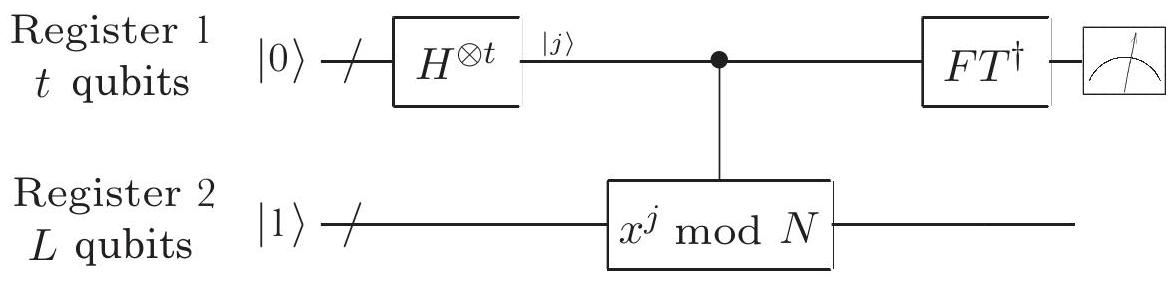
\includegraphics[width=0.75\linewidth]{Images/2024_05_17_6977ce60de6fd27aef98g-263}
\end{figure}

Figure 5.4. Quantum circuit for the order-finding algorithm. The second register is shown as being initialized to the $|1\rangle$ state, but if the method of Exercise 5.14 is used, it can be initialized to $|0\rangle$ instead. This circuit can also be used for factoring, using the reduction given in Section 5.3.2.

\subsubsection{The Continued Fraction Expansion}

The reduction of order-finding to phase estimation is completed by describing how to obtain the desired answer, $r$, from the result of the phase estimation algorithm, $\varphi \approx s / r$. We only know $\varphi$ to $2 L+1$ bits, but we also know a priori that it is a rational number - the ratio of two bounded integers - and if we could compute the nearest such fraction to $\varphi$ we might obtain $r$.

Remarkably, there is an algorithm which accomplishes this task efficiently, known as the continued fractions algorithm. An example of how this works is described in Box 5.3. The reason this algorithm satisfies our needs is the following theorem, which is proved in Appendix 4:

Theorem 5.1: Suppose $s / r$ is a rational number such that

\begin{equation}
    \left|\frac{s}{r}-\varphi\right| \leq \frac{1}{2 r^{2}} \tag{5.48}
\end{equation}

Then $s / r$ is a convergent of the continued fraction for $\varphi$, and thus can be computed in $O\left(L^{3}\right)$ operations using the continued fractions algorithm.

Since $\varphi$ is an approximation of $s / r$ accurate to $2 L+1$ bits, it follows that $|s / r-\varphi| \leq$ $2^{-2 L-1} \leq 1 / 2 r^{2}$, since $r \leq N \leq 2^{L}$. Thus, the theorem applies.

Summarizing, given $\varphi$ the continued fractions algorithm efficiently produces numbers $s^{\prime}$ and $r^{\prime}$ with no common factor, such that $s^{\prime} / r^{\prime}=s / r$. The number $r^{\prime}$ is our candidate for the order. We can check to see whether it is the order by calculating $x^{r^{\prime}} \bmod N$, and seeing if the result is 1 . If so, then $r^{\prime}$ is the order of $x$ modulo $N$, and we are done!

\subsubsection{Performance}
How can the order-finding algorithm fail? There are two possibilities. First, the phase estimation procedure might produce a bad estimate to $s / r$. This occurs with probability at most $\epsilon$, and can be made small with a negligible increase in the size of the circuit. More seriously, it might be that $s$ and $r$ have a common factor, in which case the number $r^{\prime}$ returned by the continued fractions algorithm be a factor of $r$, and not $r$ itself. Fortunately, there are at least three ways around this problem.

Perhaps the most straightforward way is to note that for randomly chosen $s$ in the range 0 through $r-1$, it's actually pretty likely that $s$ and $r$ are co-prime, in which case the continued fractions algorithm must return $r$. To see that this is the case, note that by Problem 4.1 on page 638 the number of prime numbers less than $r$ is at least

\textbf{Box 5.3: The continued fractions algorithm}

The idea of the continued fractions algorithm is to describe real numbers in terms of integers alone, using expressions of the form

\begin{equation}
    \left[a_{0}, \ldots, a_{M}\right] \equiv a_{0}+\frac{1}{a_{1}+\frac{1}{a_{2}+\frac{1}{\cdots+\frac{1}{a_{M}}}}} \tag{5.49}
\end{equation}

where $a_{0}, \ldots, a_{M}$ are positive integers. (For applications to quantum computing it is convenient to allow $a_{0}=0$ as well.) We define the $m$ th convergent $(0 \leq m \leq M)$ to this continued fraction to be $\left[a_{0}, \ldots, a_{m}\right]$. The continued fractions algorithm is a method for determining the continued fraction expansion of an arbitrary real number. It is easily understood by example. Suppose we are trying to decompose $31 / 13$ as a continued fraction. The first step of the continued fractions algorithm is to split $31 / 13$ into its integer and fractional part,

\begin{equation}
    \frac{31}{13}=2+\frac{5}{13} . \tag{5.50}
\end{equation}

Next we invert the fractional part, obtaining

\begin{equation}
    \frac{31}{13}=2+\frac{1}{\frac{13}{5}} \tag{5.51}
\end{equation}

These steps - split then invert - are now applied to $13 / 5$, giving

\begin{equation}
    \frac{31}{13}=2+\frac{1}{2+\frac{3}{5}}=2+\frac{1}{2+\frac{1}{\frac{5}{3}}} \tag{5.52}
\end{equation}

Next we split and invert $5 / 3$ :

\begin{equation}
    \frac{31}{13}=2+\frac{1}{2+\frac{1}{1+\frac{1}{3}}}=2+\frac{1}{2+\frac{1}{1+\frac{1}{2}}} \tag{5.53}
\end{equation}

The decomposition into a continued fraction now terminates, since

\begin{equation}
    \frac{3}{2}=1+\frac{1}{2} \tag{5.54}
\end{equation}

may be written with a 1 in the numerator without any need to invert, giving a final continued fraction representation of $31 / 13$ as

\begin{equation}
    \frac{31}{13}=2+\frac{1}{2+\frac{1}{1+\frac{1}{1+\frac{1}{2}}}} \tag{5.55}
\end{equation}

It's clear that the continued fractions algorithm terminates after a finite number of 'split and invert' steps for any rational number, since the numerators which appear ( $31,5,3,2,1$ in the example) are strictly decreasing. How quickly does this termination occur? It turns out that if $\varphi=s / r$ is a rational number, and $s$ and $r$ are $L$ bit integers, then the continued fraction expansion for $\varphi$ can be computed using $O\left(L^{3}\right)$ operations $-O(L)$ 'split and invert' steps, each using $O\left(L^{2}\right)$ gates for elementary arithmetic.\\
$r / 2 \log r$, and thus the chance that $s$ is prime (and therefore, co-prime to $r$ ) is at least $1 / 2 \log (r)>1 / 2 \log (N)$. Thus, repeating the algorithm $2 \log (N)$ times we will, with high probability, observe a phase $s / r$ such that $s$ and $r$ are co-prime, and therefore the continued fractions algorithm produces $r$, as desired.

A second method is to note that if $r^{\prime} \neq r$, then $r^{\prime}$ is guaranteed to be a factor of $r$, unless $s=0$, which possibility occurs with probability $1 / r \leq 1 / 2$, and which can be discounted further by a few repetitions. Suppose we replace $a$ by $a^{\prime} \equiv a^{r^{\prime}}(\bmod N)$. Then the order of $a^{\prime}$ is $r / r^{\prime}$. We can now repeat the algorithm, and try to compute the order of $a^{\prime}$, which, if we succeed, allows us to compute the order of $a$, since $r=r^{\prime} \times r / r^{\prime}$. If we fail, then we obtain $r^{\prime \prime}$ which is a factor of $r / r^{\prime}$, and we now try to compute the order of $a^{\prime \prime} \equiv\left(a^{\prime}\right)^{r^{\prime \prime}}(\bmod N)$. We iterate this procedure until we determine the order of a. At most $\log (r)=O(L)$ iterations are required, since each repetition reduces the order of the current candidate $a^{\prime \prime} \cdots$ by a factor of at least two.

The third method is better than the first two methods, in that it requires only a constant number of trials, rather than $O(L)$ repetitions. The idea is to repeat the phase estimation-continued fractions procedure twice, obtaining $r_{1}^{\prime}, s_{1}^{\prime}$ the first time, and $r_{2}^{\prime}, s_{2}^{\prime}$ the second time. Provided $s_{1}^{\prime}$ and $s_{2}^{\prime}$ have no common factors, $r$ may be extracted by taking the least common multiple of $r_{1}$ and $r_{2}$. The probability that $s_{1}^{\prime}$ and $s_{2}^{\prime}$ have no common factors is given by

\begin{equation}
    1-\sum_{q} p\left(q \mid s_{1}^{\prime}\right) p\left(q \mid s_{2}^{\prime}\right) \tag{5.56}
\end{equation}

where the sum is over all prime numbers $q$, and $p(x \mid y)$ here means the probability of $x$ dividing $y$. If $q$ divides $s_{1}^{\prime}$ then it must also divide the true value of $s, s_{1}$, on the first iteration, so to upper bound $p\left(q \mid s_{1}^{\prime}\right)$ it suffices to upper bound $p\left(q \mid s_{1}\right)$, where $s_{1}$ is chosen uniformly at random from 0 through $r-1$. It is easy to see that $p\left(q \mid s_{1}\right) \leq 1 / q$, and thus $p\left(q \mid s_{1}^{\prime}\right) \leq 1 / q$. Similarly, $p\left(q \mid s_{2}^{\prime}\right) \leq 1 / q$, and thus the probability that $s_{1}^{\prime}$ and $s_{2}^{\prime}$ have no common factors satisfies

\begin{equation}
    1-\sum_{q} p\left(q \mid s_{1}^{\prime}\right) p\left(q \mid s_{2}^{\prime}\right) \geq 1-\sum_{q} \frac{1}{q^{2}} \tag{5.57}
\end{equation}

The right hand side can be upper bounded in a number of ways; a simple technique is provided in Exercise 5.16, which gives

\begin{equation}
    1-\sum_{q} p\left(q \mid s_{1}^{\prime}\right) p\left(q \mid s_{2}^{\prime}\right) \geq \frac{1}{4} \tag{5.58}
\end{equation}

and thus the probability of obtaining the correct $r$ is at least $1 / 4$.

Exercise 5.15: Show that the least common multiple of positive integers $x$ and $y$ is $x y / \operatorname{gcd}(x, y)$, and thus may be computed in $O\left(L^{2}\right)$ operations if $x$ and $y$ are $L$ bit numbers.

Exercise 5.16: For all $x \geq 2$ prove that $\int_{x}^{x+1} 1 / y^{2} d y \geq 2 / 3 x^{2}$. Show that

\begin{equation}
    \sum_{q} \frac{1}{q^{2}} \leq \frac{3}{2} \int_{2}^{\infty} \frac{1}{y^{2}} d y=\frac{3}{4} \tag{5.59}
\end{equation}

and thus that $(5.58)$ holds.

What resource requirements does this algorithm consume? The Hadamard transform requires $O(L)$ gates, and the inverse Fourier transform requires $O\left(L^{2}\right)$ gates. The major cost in the quantum circuit proper actually comes from the modular exponentiation, which uses $O\left(L^{3}\right)$ gates, for a total of $O\left(L^{3}\right)$ gates in the quantum circuit proper. The continued fractions algorithm adds $O\left(L^{3}\right)$ more gates, for a total of $O\left(L^{3}\right)$ gates to obtain $r^{\prime}$. Using the third method for obtaining $r$ from $r^{\prime}$ we need only repeat this procedure a constant number of times to obtain the order, $r$, for a total cost of $O\left(L^{3}\right)$. The algorithm is summarized below.

\textbf{Algorithm: Quantum order-finding}

Inputs: (1) A black box $U_{x, N}$ which performs the transformation $|j\rangle|k\rangle \rightarrow|j\rangle\left|x^{j} k \bmod N\right\rangle$, for $x$ co-prime to the $L$-bit number $N$, (2) $t=2 L+1+\left\lceil\log \left(2+\frac{1}{2 \epsilon}\right)\right\rceil$ qubits initialized to $|0\rangle$, and (3) $L$ qubits initialized to the state $|1\rangle$.

Outputs: The least integer $r>0$ such that $x^{r}=1(\bmod N)$.

Runtime: $O\left(L^{3}\right)$ operations. Succeeds with probability $O(1)$.

\textbf{Procedure:}
\begin{enumerate}
    \item $\quad|0\rangle|1\rangle$
    \item $\rightarrow \frac{1}{\sqrt{2^{t}}} \sum_{j=0}^{2^{t}-1}|j\rangle|1\rangle$
    \item $\rightarrow \frac{1}{\sqrt{2^{t}}} \sum_{j=0}^{2^{t}-1}|j\rangle\left|x^{j} \bmod N\right\rangle$

\end{enumerate}

$\approx \frac{1}{\sqrt{r 2^{t}}} \sum_{s=0}^{r-1} \sum_{j=0}^{2^{t}-1} e^{2 \pi i s j / r}|j\rangle\left|u_{s}\right\rangle$

\begin{enumerate}
  \setcounter{enumi}{3}
    \item $\quad \rightarrow \frac{1}{\sqrt{r}} \sum_{s=0}^{r-1}|\widetilde{s / r}\rangle\left|u_{s}\right\rangle$
    \item $\rightarrow \widetilde{s / r}$
    \item $\rightarrow r$ initial state

\end{enumerate}

create superposition

apply $U_{x, N}$

apply inverse Fourier transform to first register

measure first register

apply continued fractions algorithm

\subsection{5.3.2 Application: Factoring}
The problem of distinguishing prime numbers from composites, and of resolving composite numbers into their prime factors, is one of the most important and useful in all of arithmetic. [ ...] The dignity of science seems to demand that every aid to the solution of such an elegant and celebrated problem be zealously cultivated.

\begin{itemize}
    \item Carl Friedrich Gauss, as quoted by Donald Knuth
\end{itemize}

Given a positive composite integer $N$, what prime numbers when multiplied together equal it? This factoring problem turns out to be equivalent to the order-finding problem\\
we just studied, in the sense that a fast algorithm for order-finding can easily be turned into a fast algorithm for factoring. In this section we explain the method used to reduce factoring to order-finding, and give a simple example of this reduction.

The reduction of factoring to order-finding proceeds in two basic steps. The first step is to show that we can compute a factor of $N$ if we can find a non-trivial solution $x \neq \pm 1(\bmod N)$ to the equation $x^{2}=1(\bmod N)$. The second step is to show that a randomly chosen $y$ co-prime to $N$ is quite likely to have an order $r$ which is even, and such that $y^{r / 2} \neq \pm 1(\bmod N)$, and thus $x \equiv y^{r / 2}(\bmod N)$ is a non-trivial solution to $x^{2}=1(\bmod N)$. These two steps are embodied in the following theorems, whose proofs may be found in Section A4.3 of Appendix 4.

Theorem 5.2: Suppose $N$ is an $L$ bit composite number, and $x$ is a non-trivial solution to the equation $x^{2}=1(\bmod N)$ in the range $1 \leq x \leq N$, that is, neither $x=1(\bmod N)$ nor $x=N-1=-1(\bmod N)$. Then at least one of $\operatorname{gcd}(x-1, N)$ and $\operatorname{gcd}(x+1, N)$ is a non-trivial factor of $N$ that can be computed using $O\left(L^{3}\right)$ operations.

Theorem 5.3: Suppose $N=p_{1}^{\alpha_{1}} \ldots p_{m}^{\alpha_{m}}$ is the prime factorization of an odd composite positive integer. Let $x$ be an integer chosen uniformly at random, subject to the requirements that $1 \leq x \leq N-1$ and $x$ is co-prime to $N$. Let $r$ be the order of $x$ modulo $N$. Then

\begin{equation}
    p\left(r \text { is even and } x^{r / 2} \neq-1(\bmod N)\right) \geq 1-\frac{1}{2^{m}} \tag{5.60}
\end{equation}

Theorems 5.2 and 5.3 can be combined to give an algorithm which, with high probability, returns a non-trivial factor of any composite $N$. All the steps in the algorithm can be performed efficiently on a classical computer except (so far as is known today) an order-finding 'subroutine' which is used by the algorithm. By repeating the procedure we may find a complete prime factorization of $N$. The algorithm is summarized below.

\textbf{Algorithm: Reduction of factoring to order-finding}
Inputs: A composite number $N$

Outputs: A non-trivial factor of $N$.

Runtime: $O\left((\log N)^{3}\right)$ operations. Succeeds with probability $O(1)$.

\textbf{Procedure:}
\begin{enumerate}
    \item If $N$ is even, return the factor 2 .
    \item $\quad$ Determine whether $N=a^{b}$ for integers $a \geq 1$ and $b \geq 2$, and if so return the factor $a$ (uses the classical algorithm of Exercise 5.17).
    \item Randomly choose $x$ in the range 1 to $N-1$. If $\operatorname{gcd}(x, N)>1$ then return the factor $\operatorname{gcd}(x, N)$.
    \item Use the order-finding subroutine to find the order $r$ of $x$ modulo $N$.
    \item If $r$ is even and $x^{r / 2} \neq-1(\bmod N)$ then compute $\operatorname{gcd}\left(x^{r / 2}-1, N\right)$ and $\operatorname{gcd}\left(x^{r / 2}+1, N\right)$, and test to see if one of these is a non-trivial factor, returning that factor if so. Otherwise, the algorithm fails.

\end{enumerate}

Steps 1 and 2 of the algorithm either return a factor, or else ensure that $N$ is an odd integer with more than one prime factor. These steps may be performed using $O(1)$ and $O\left(L^{3}\right)$ operations, respectively. Step 3 either returns a factor, or produces a randomly chosen element $x$ of $\{0,1,2, \ldots, N-1\}$. Step 4 calls the order-finding subroutine, computing the order $r$ of $x$ modulo $N$. Step $\mathbf{5}$ completes the algorithm, since Theorem 5.3 guarantees that with probability at least one-half $r$ will be even and $x^{r / 2} \neq-1(\bmod N)$, and then Theorem 5.2 guarantees that either $\operatorname{gcd}\left(x^{r / 2}-1, N\right)$ or $\operatorname{gcd}\left(x^{r / 2}+1, N\right)$ is a non-trivial factor of $N$. An example illustrating the use of this algorithm with the quantum order-finding subroutine is shown in Box 5.4.

Exercise 5.17: Suppose $N$ is $L$ bits long. The aim of this exercise is to find an efficient classical algorithm to determine whether $N=a^{b}$ for some integers $a \geq 1$ and $b \geq 2$. This may be done as follows:

(1) Show that $b$, if it exists, satisfies $b \leq L$.

(2) Show that it takes at most $O\left(L^{2}\right)$ operations to compute $\log _{2} N, x=y / b$ for $b \leq L$, and the two integers $u_{1}$ and $u_{2}$ nearest to $2^{x}$.

(3) Show that it takes at most $O\left(L^{2}\right)$ operations to compute $u_{1}^{b}$ and $u_{2}^{b}$ (use repeated squaring) and check to see if either is equal to $N$.

(4) Combine the previous results to give an $O\left(L^{3}\right)$ operation algorithm to determine whether $N=a^{b}$ for integers $a$ and $b$.

Exercise 5.18: (Factoring 91) Suppose we wish to factor $N=91$. Confirm that steps $\mathbf{1}$ and $\mathbf{2}$ are passed. For step 3, suppose we choose $x=4$, which is co-prime to 91 . Compute the order $r$ of $x$ with respect to $N$, and show that $x^{r / 2} \bmod 91=64 \neq-1(\bmod 91)$, so the algorithm succeeds, giving $\operatorname{gcd}(64-1,19)=7$.

It is unlikely that this is the most efficient method you've seen for factoring 91. Indeed, if all computations had to be carried out on a classical computer, this reduction would not result in an efficient factoring algorithm, as no efficient method is known for solving the order-finding problem on a classical computer.

Exercise 5.19: Show that $N=15$ is the smallest number for which the order-finding subroutine is required, that is, it is the smallest composite number that is not even or a power of some smaller integer.